\documentclass[fleqn]{jbook}
\usepackage{physpub}

\begin{document}
\begin{question}{問題7}{佐藤光浩}
 高エネルギー加速器からの陽子ビームを金属標的にあてると、正に帯電した二
次粒子として$K$中間子の他、$\pi$中間子、$\mu$粒子などが作られる。このう
ち、正に帯電した$K$中間子をビームラインに誘導することを考える。荷電$K$中
間子、荷電$\pi$中間子、中性$\pi$中間子の質量はそれぞれ、$494MeV/c^2$、
$135MeV/c^2$である。光速$c$は$3.0\times 10^8m/s$とする。全問にわたり、数
値計算は有効数字$2$桁で求めよ。

金属標的で作られた二次粒子に、進行方向に垂直な磁場を与えると、運動量に比
例した軌道半径の円運動をする。$1.0GeV/c$の$K$中間子を取り出すつもりで当
てた磁場で、$K$中間子以外の粒子にも同じ軌道を飛行するものがある。磁場を
通過した後、進行方向と垂直に一様電場を加えることで粒子を種類別に振り分け
ることができる。質量$m$、運動量$\mathbf{p}$の荷電粒子(電荷$e$を持つ)が電場$\mathbf{E}$中を通
過するとき、相対論的な運動方程式$d\mathbf{p}/dt=e\mathbf{E}$を満たす。

\begin{enumerate}

\item
図$1$のように、この荷電粒子が電場領域に入射する方向を$y$軸、それに垂直な
電場の方向を$x$軸にとる。荷電粒子が電場領域に入射したときの運動量を
$\mathbf{p_0}$とする。電場領域に入射したときから時間$t$経過した後の荷電
粒子のエネルギー$\epsilon$を求めよ。

\begin{figure}[htbp]
  \begin{center}
    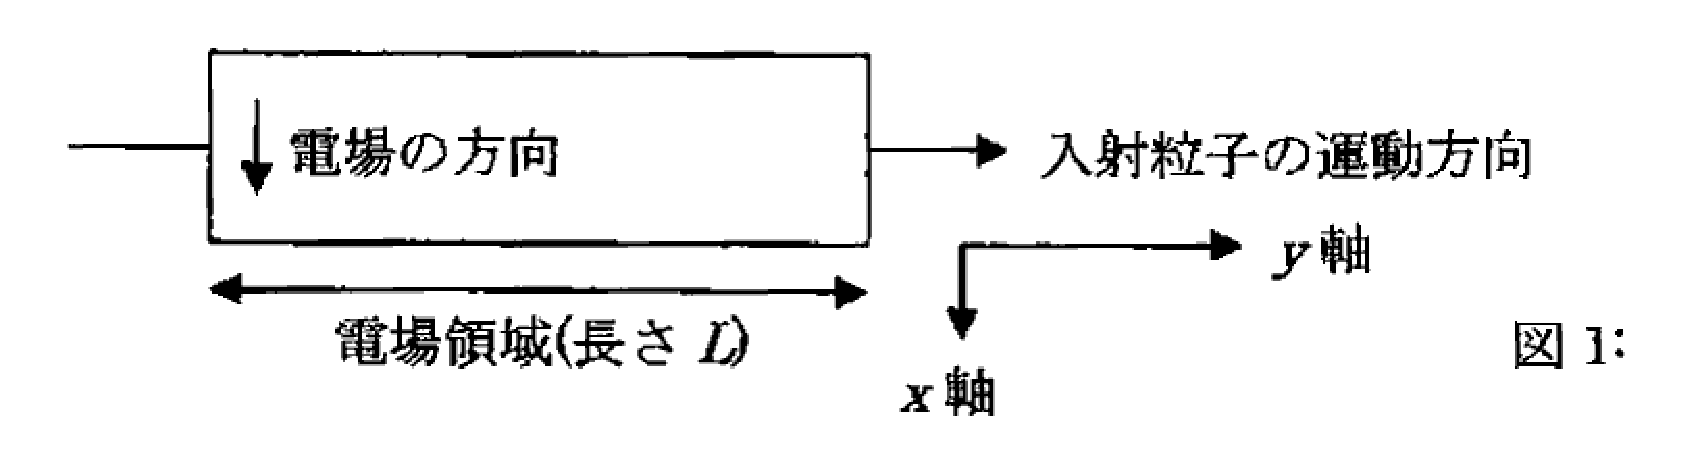
\includegraphics[width=150mm]{2003phy7-1.eps}
  \end{center}
  \ilabel{fig:2003phy7-1}
\end{figure}

\item
一般に荷電粒子のエネルギー$\epsilon$、運動量$\mathbf{p}$と速度
$\mathbf{v}$には$\mathbf{v}=\mathbf{p}c^2/\epsilon$の関係がある。このこ
とを用い、さらに時間積分することにより、荷電粒子の座標$x$と$y$を求めよ。
必要ならば、積分公式$\int \frac{dx}{\sqrt{1+x^2}}=\sinh^{-1}x$を使うこと。

\item
長さ$L$の領域を出たときの荷電粒子の進行方向が$y$軸となす角度を求めよ。

\item
ふれ角度が十分小さいとして、荷電$K$中間子のふれ角に比べ、同じ
$1.0GeV/c$の運動量で入射した荷電$\pi$中間子のふれ角はおよそどのくらいに
なるか。
\end{enumerate}

K中間子を金属に入射し、その中で完全に停止させる。荷電$K$中間子は$63\%$が
$\mu$粒子と$\mu$型ニュートリノに、$21\%$が荷電$\pi$中間子と中性$\pi$中間子
($\pi^0$)に二体崩壊する。ここでは$\pi$中間子への崩壊に着目する。

中性$\pi$中間子は$\tau=8.4\times 10^{-17}$秒という非常に短い時間に崩壊し、
2つのガンマ線になる。実験室系で見たときの中性$\pi$中間子の静止座標系の移
動速度を$\mathbf{v}$とする。二つの系の間のローレンツ変換は
$p^{\prime}\sin \theta^{\prime} = p\sin \theta$および$p^{\prime} \cos
\theta^{\prime}=p\cos \theta \cdot \gamma -E\gamma\beta/c$ で与えられる。
ここで$\beta \equiv \frac{v}{c}$、$\gamma \equiv
\frac{1}{1-\frac{v^2}{c^2}}$である。$\prime$がついたものは重心系、そうで
はないものは実験室系を表す。$\theta$および、$\theta^{\prime}$はそれぞれ
の系でび粒子の運動方向が静止座標系の移動方向となす角度を表す。

\begin{enumerate}\setcounter{enumi}{4}
\item
 中性$\pi$中間子の進行方向を$x$軸にとるとき、2つのガンマ線がx軸について
対称な方向に等しい運動量の絶対値をもって放出されたとする。このときガン
マ線がx軸となす角度を計算せよ。$\beta$を用いてよい。
\end{enumerate}

上述のように中性$\pi$中間子の寿命$\tau$は非常に短い。この寿命をどのよう
に測定するかを考えよう。

\begin{enumerate}\setcounter{enumi}{5}
\item
 実験室で中性$\pi$中間子が飛行中に崩壊する。作られてから崩壊するまでの平
均距離が$25$ミクロン程度となるためには、生成された中性$\pi$中間子のエネ
ルギーはどのようなものでないといけないか。
\end{enumerate}

中性$\pi$中間子は電磁相互作用をしないが、崩壊生成物であるガンマ線は物質
中で対生成を起す。$2$枚の金属薄膜を近接しておき、高エネルギー陽子ビーム
を当てると、薄膜中で中性$\pi$中間子が作られる。最初の薄膜中で生成された
中性$\pi$中間子は短い距離をとんだ後崩壊し、$2$個のガンマ線になる。ガンマ
線になると一定の確率で、金属薄膜中で対生成を起す。図$2$にあるように、一
枚目の薄膜中で中性$\pi$中間子が作られ、薄膜の間で崩壊し、$2$枚目の薄膜中
で対生成を起すものに着目する。

\begin{figure}[htbp]
  \begin{center}
    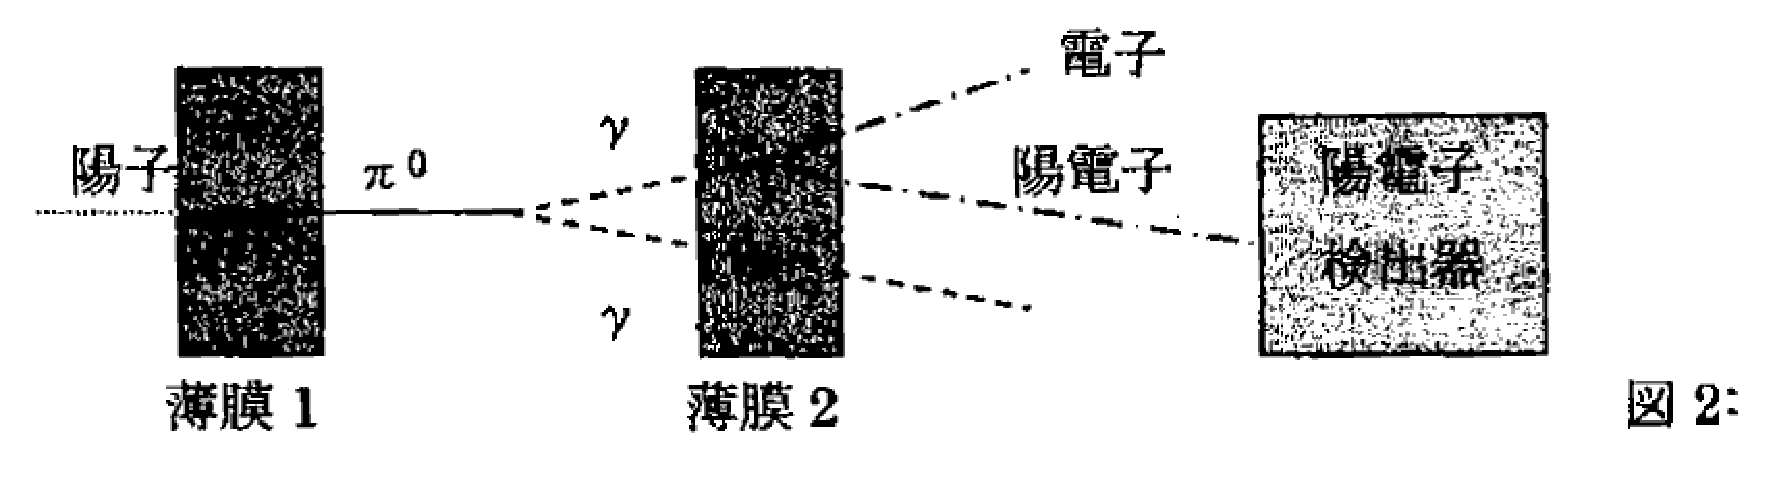
\includegraphics[width=150mm]{2003phy7-2.eps}
  \end{center}
  \ilabel{fig:2003phy7-2}
\end{figure}

\begin{enumerate}\setcounter{enumi}{6}
\item
 対生成で生じた陽電子をビーム進行方向の陽電子検出器で観測する。まず、2枚
の薄膜を再接近させた状態で陽電子を計測し、その後、薄膜間の距離を$d$だけ
増やして計測するよ。このときの陽電子の計測率の変化について説明せよ。

\item 
 薄膜間の距離の変化に対する感度を最も高くするためには、薄膜の厚さはどう
とるべきか考察せよ。

\end{enumerate}
\end{question}

\begin{answer}{問題7}{佐藤光浩}
\begin{enumerate}
    \item 
\begin{eqnarray}
 \frac{d}{dt}\left(\begin{array}{c}
 p_x \\ p_y \\ \end{array} \right)
 &= e \left(\begin{array}{c}
 E \\ 0 \\ \end{array} \right) \nonumber\\
 \left(\begin{array}{c}
 p_x(0) \\ p_y(0) \\ \end{array} \right)
 &= \left(\begin{array}{c} 
 0 \\ p_0 \\ \end{array} \right) 
\end{eqnarray}

\begin{eqnarray}
 \left(\begin{array}{c}
 p_x(t) \\ p_y(t) \\ \end{array} \right)
 = \left(\begin{array}{c}
  eEt \\ p_0 \\ \end{array} \right) 
\end{eqnarray}
Einstein's equation $\frac{\epsilon^2}{c^2} - p^2 =m^2 c^2$より、
\begin{eqnarray}
 \epsilon^2 = (c^2p^2 + m^2c^4)^{\frac{1}{2}} \\
 = \left[c^2 (p_0^2 + e^2E^2t^2) + m^2c^4\right]^{\frac{1}{2}} \ilabel{7.1}
\end{eqnarray}

    \item
$\mathbf{p} = m \gamma c \mathbf{\beta}$、$\epsilon = m \gamma c^2$より、
$\mathbf{p} = \epsilon \cdot \frac{\mathbf{\beta}}{c}$の関係式が常に成り
立っているので、$\mathbf{v} = \frac{\mathbf{p}c^2}{\epsilon}$の関係に式
(\iref{7.1})を代入して、

\begin{eqnarray}
 \left(\begin{array}{c} 
 v_x(t) \\ v_y(t) \end{array} \right)
 = \frac{c^2}{\sqrt{m^2c^4 + c^2p_0^2 + c^2e^2E^2t^2}}
 \left(\begin{array}{c}
 eEt \\ p_0 \end{array} \right) \ilabel{velosity}
\end{eqnarray}
$v_x(t)$成分を時間積分すると、
\begin{eqnarray*}
 \int^{t}_0 dt^{\prime}
 \frac{ec^2Et^{\prime}}{\sqrt{m^2c^4+c^2p_0^2+c^2e^2E^2t^{\prime 2}}}\\
 \end{eqnarray*}
ここで、$ \alpha \equiv \frac{m^2c^2 +c^2p_0^2}{c^2e^2E^2}$とおくと、
\begin{eqnarray*}
 &= \int^{t^2}_{0}dt^{\prime 2}\frac{c}{2\sqrt{t^{\prime 2} + \alpha}}\\
 &= \left[c(t^{\prime 2} +\alpha)^{\frac{1}{2}}\right]^{t^2}_0\\
 &= c \left\{ c(t^{2} +\alpha)^{\frac{1}{2}} -
 \alpha^{\frac{1}{2}} \right\} \\
\end{eqnarray*}
ここで$\alpha$を元の形に戻すと、
\begin{eqnarray*}
 = \frac{1}{eE} \left\{
 \sqrt{c^2e^2E^2t^2+(m^2c^4+c^2P_0^2)-\sqrt{m^2c^4+c^2P_0^2}}\right\}
\end{eqnarray*}
次に、$v_y(t)$成分を時間積分すると、
\begin{eqnarray*}
 \int^{t}_0 dt^{\prime}
 \frac{c^2P_0}{\sqrt{m^2c^4+c^2P_0^2+c^2e^2E^2t^2}}
\end{eqnarray*}
ここで、$ \beta = \frac{c^2e^2E^2}{m^2c^4+c^2P_0^2}$とおくと、
\begin{eqnarray*}
  &= \frac{c^2P_0/\beta}{\sqrt{m^2c^4+c^2P_0^2}} \int^t_0
  d(\beta t^{\prime}) \frac{1}{\sqrt{1+(\beta t^{\prime})^2}} \\
  &= \frac{c^2P_0/\beta}{\sqrt{m^2c^r+c^2P_0^2}} \sinh^{-1} \beta t \\
  &= \frac{cP_0}{eE} sinh^{-1}
  \left(\frac{ceEt}{\sqrt{m^2c^4+c^2P_0^2}} \right) \\
\end{eqnarray*}
以上から、
\begin{eqnarray}
 \left(\begin{array}{c} x\\ y\end{array} \right) = \left(\begin{array}{c}
 \frac{1}{eE}
 \left(\sqrt{(m^2c^4+c^2P_0^2)+(ceEt)^2}-\sqrt{m^2c^4+c^2P_0^2} \right) \\
  \frac{cP_0}{eE}
 \sinh^{-1}\left(\frac{ceEt}{\sqrt{m^2c^4+c^2P_0^2}}\right) \end{array}
\right) \ilabel{coordinate}
\end{eqnarray}

    \item
 $y=L$のとき、$\tan\theta = \frac{v_x}{v_y} \rightarrow \theta =
\tan^{-1} \left(\frac{v_x}{v_y}\right)$であるから、

まず、$t$と$L$の関係は(\iref{coordinate})から、
\begin{eqnarray*}
 L = \frac{cp}{eE} \sinh^{-1} \left(\frac{ceEt}{\sqrt{m^2c^4+c^2P_0^2}}\right)
\end{eqnarray*}
であり、(\iref{velosity})から$\frac{v_x}{v_y}$も求まり、上式とあわせて
\begin{eqnarray*}
  \frac{v_x}{v_y} = \frac{cEt}{P_0} 
  = \frac{\sqrt{m^2c^4 + c^2P_0^2}}{cP_0}\sinh
  \left(\frac{eEL}{cP_0}\right) 
\end{eqnarray*}
ゆえに、
\begin{eqnarray}
 \theta = \tan^{-1}
 \left[\frac{\sqrt{m^2c^4+c^2P_0^2}{cP_0}}\sinh(\frac{eEL}{cP_p})\right]
 \\
\end{eqnarray}

    \item
 揺れ角が十分小さいときには$\theta \sim \frac{v_x}{v_y}$と近似してよい。

\begin{eqnarray*}
 \theta = \left(1+\frac{m^2c^2}{P_0^2}\right)^{\frac{1}{2}}
 \sinh\left(\frac{eEL}{cP_0}\right)
\end{eqnarray*}

$P_0=1.0[Gev]$、$m_{\kappa}=494[Mev/c^2]$、$m_{\pi}=140[Mev/c^2]$を用いて、
\begin{eqnarray}
  \frac{\theta_{\pi}}{\theta_{\kappa}} &\sim
  \frac{\left(1+\frac{m_{\pi}^2c^2}{P_0}\right)^{\frac{1}{2}}}{\left(1+\frac{m_{\kappa}^2c^2}{P_0}\right)^{\frac{1}{2}}} 
  = \left(\frac{1+0.140^2}{1+0.494^2}\right)^{\frac{1}{2}} \\
 &\simeq 0.91 \\
\end{eqnarray}

    \item
$\pi^0$の静止系(実験室系を基準として$\pi^0$静止系に$\prime$をつける)で崩
壊をみると崩壊$\pi^0 \rightarrow \gamma\gamma$のエネ
ルギー保存則と運動量保存則は、

\begin{eqnarray}
 \begin{cases}
  \text{エネルギー保存則} m_{\pi^0}c^2 = c{P_1}^{\prime} + c{P_2}^{\prime}
  \\
  \text{運動量保存則} 0 = \mathbf{P_1}^{\prime} + \mathbf{P_2}^{\prime}
  \\
 \end{cases}
\end{eqnarray}
$\gamma$線が$x$軸に対して対称に運動しているのだから、$x^{\prime}$軸に対し
ても対称に運動するはずである。また、運動量保存則から$\gamma$線は$\pi^0$
静止系では反対向きに飛び散る。よって、
$\mathbf{P_1^{\prime}}=P_y^{\prime}\mathbf{y^{\prime}}$、
$\mathbf{P_2^{\prime}}=-P_y^{\prime}\mathbf{y^{\prime}}$であるから、

\begin{eqnarray*}
 m_{\pi^0} = 2 P_{y^{\prime}} \hspace{15pt} ie. P_{y^{\prime}} =
 \frac{m_{\pi^0}c}{2}
\end{eqnarray*}

$4$元運動量$(\frac{\epsilon}{c},P_x,P_y,P_z)$は反変ベクトルなので
$\mathbf{P_{{\gamma}_1}}^{\mu^{\prime}}
=\left(\frac{m_{{\pi}_0}c}{2},0,\frac{m_{{\pi}_0}c}{2},0\right)$、
$\mathbf{P_{{\gamma}_2}}^{\mu^{\prime}}
=\left(\frac{m_{{\pi}_0}c}{2},0,-\frac{m_{{\pi}_0}c}{2},0\right)$
である。これを実験室系に戻すと、

\begin{eqnarray*}
 \mathbf{P^{{\mu}^{\prime}}} = \Lambda^{{\mu}^{\prime}}_{\nu}
 \mathbf{P^{\nu}} \hspace{15pt} ie. \mathbf{P^{\nu}} =
 \left(\Lambda^{{\mu}^{\prime}}_{\nu} \right)^{-1}
 \mathbf{P^{{\mu}^{\prime}}} 
\end{eqnarray*}
matrix表示では、
\begin{eqnarray*}
 \left[\begin{array}{c} \frac{\epsilon}{c} \\ P_x\\ P_y\\ P_z
       \end{array} \right] 
 &= \left(\begin{array}{c c c c} \gamma & -\gamma\beta & 0 & 0 \\
 -\gamma\beta & \gamma & 0 & 0 \\ 0 & 0 & 1 & 0 \\ 0 & 0 & 0 & 1 \end{array}
   \right) 
   \left[\begin{array}{c} \frac{\epsilon^{\prime}}{c} \\ {P_x}^{\prime}\\
 {P_y}^{\prime}\\ {P_z}^{\prime}
   \end{array} \right] \\
 &= \left(\begin{array}{c c c c} \gamma & \gamma\beta & 0 & 0 \\
 \gamma\beta & \gamma & 0 & 0 \\ 0 & 0 & 1 & 0 \\ 0 & 0 & 0 & 1 \end{array}
   \right) 
   \left[\begin{array}{c} \frac{\epsilon^{\prime}}{c} \\ {P_x}^{\prime}\\
 {P_y}^{\prime}\\ {P_z}^{\prime}
   \end{array} \right] \\
 &= \left[\begin{array}{c} \frac{m_{{\pi}_0}\gamma c}{2} \\
 \frac{m_{{\pi}_0}\gamma \beta c}{2} \\ \frac{m_{{\pi}_0}c}{2} \\
 0\end{array}
 \right]
\end{eqnarray*}

$\gamma_{2}$について同様に計算すれば、$y$成分が反転した結果を得る。
\begin{eqnarray}
 \mathbf{P_{\gamma_{1}}} 
= \left[\begin{array}{c} \frac{m_{{\pi}_0}\gamma c}{2} \\
 \frac{m_{{\pi}_0}\gamma \beta c}{2} \\ \frac{m_{{\pi}_0}c}{2} \\
 0\end{array}
 \right] \hspace{20pt} \mathbf{P_{\gamma_{2}}}
 = \left[\begin{array}{c} \frac{m_{{\pi}_0}\gamma c}{2} \\
 \frac{m_{{\pi}_0}\gamma \beta c}{2} \\ -\frac{m_{{\pi}_0}c}{2} \\
 0\end{array} \right]
\end{eqnarray}

$\gamma$線が$x$軸となす角度は$\tan \theta = \frac{|v_y|}{|v_x|} =
\frac{1}{\gamma \beta}$より、$\theta= \tan^{-1}\left(\frac{1}{\gamma
\beta}\right)$である。

    \item
$\pi^{0}$静止系での$\tau^{\prime}=8.4\times10^{-17}sec$は実験室系では
$\tau = \gamma \tau^{\prime}$である。$v$一定として、
$\gamma\tau^{\prime}$時間にすすむ距離は$v\gamma\tau^{\prime}=25\mu m$で
あるから、$\gamma=\frac{\beta \tau^{\prime}}{\sqrt{1-\beta^2}}$を代入し
て、
\begin{eqnarray*}
 \frac{c\beta \tau^{\prime}}{\sqrt{1-\beta^2}} = 25 \times 10^{-6} sec
\end{eqnarray*}
簡単のために以下の置き換えを行えば、
\begin{eqnarray*}
 A \equiv \frac{25 \times 10^{-6}sec}{c \tau^{\prime}} = 995 sec/m 
 \hspace{20pt}
 \beta^2 = \frac{A^2}{1+A^2} \\
\end{eqnarray*}
よって、中性$\gamma$線のエネルギーは
\begin{eqnarray}
 \epsilon &= \frac{mc^2}{\sqrt{1-\beta^2}} = \frac{mc^2}{1 -
 \frac{A^2}{1+A^2}}
 \simeq \sqrt{1+A^2}mc^2 \simeq Amc^2 \\
 &\simeq 1.3 \times 10^9 eV
\end{eqnarray}

    \item
 空気中での$\gamma$線の減衰長を$X_{air}$とおき、簡単のため$\pi^0
\rightarrow \gamma \gamma$の崩壊機構を問題5で指定された方向の$\gamma$線
絞って考える。薄膜を距離$d$だけ離すことによって$\gamma$線が大気中を余計
に走ることになる距離は$d\sqrt{1+\frac{1}{\beta^2\gamma^2}}$であるから、
$\gamma$線の輸送方程式、

\begin{eqnarray}
 \frac{N_{\gamma}}{x} = -\frac{N_{\gamma}}{X_{air}}
\end{eqnarray}
をといて、$N_{\text{薄膜2}} =
N_0(1-e^{-\frac{d \sqrt{1+\frac{1}{\beta^2\gamma^2}}}{X_{air}}})$であるので、
その後の$\gamma \rightarrow e^{+}e^{-}$の対生成過程で電子が飛んで検出器
の方向に出てゆくものの粒子分布は同一とみなせるので陽電子の検出器における
計測率は$1-e^{-\frac{d \sqrt{1+\frac{1}{\beta^2\gamma^2}}}{X_{air}}}$倍になる。

    \item
 薄膜2中で起こる反応は2つある。1つは$\gamma$線からの対生成、また2つめは
対生成された陽電子が金属中の電子と対消滅を起す反応である。簡単のために薄
膜中を走る距離を薄膜自身の厚さ($L$)と同じとする。次に薄膜2中の、対生成による
$\gamma$線の減衰長を$X_{\gamma}$、対消滅による陽電子線の減衰長を
$X_{e^{+}}$とおけば、薄膜2中$l$の距離で$\gamma$線が崩壊したものの粒子数
は前問の$N_{\text{薄膜2}}$を用いて、

\begin{eqnarray}
 N_{\text{薄膜2を出て行く陽電子数}} &= \Sigma_{l} N_{\text{薄膜2}}
 e^{-\frac{l}{X_{\gamma}}} \left( 1- e^{\frac{L-l}{X_{e^{+}}}}\right) \\\
 &= \int_{0}{L} dl N_{\text{薄膜2}}
 e^{-\frac{l}{X_{\gamma}}} \left( 1- e^{\frac{L-l}{X_{e^{+}}}}\right)  \\\
 &=  N_{\text{薄膜2}}
 \left[X_{\gamma}\left(1-e^{-\frac{L}{X_{\gamma}}}\right)
- \frac{X_{e^{+}}X_{\gamma}}{X_{e^{+}}-X_{\gamma}}
 \left(e^{-\frac{L}{X_{e^{+}}}} -
 e^{-\frac{L}{X_{\gamma}}}\right)\right] 
\end{eqnarray}

よって、これが最大となるような$L$にすればよい。よって陽電子の消滅が
$\gamma$線の崩壊よりdominantな薄膜ではなるべく薄く、陽電子の消滅より
$\gamma$線の崩壊が十分な薄膜ではなるべく厚くすればよい。

\end{enumerate}
\end{answer}
\end{document}
